\section{Topologies of real-time multimedia communication}
\label{sec:topologies}


%% 
%% Leave first page empty
\thispagestyle{empty}

This chapter will discuss different possible topologies that can be used along in real time media communication.

A topology can be defined as the arrangement of the various nodes of a network together, those nodes can be connected through different links and configurations. Topologies may have different logics and paths to have optimal performance for each specific scenario. In WebRTC, we want to study how they perform in the most common use cases for real time multimedia communication.

Some challenges will be common in all the topologies described in this chapter. For example, NAT traversal problems will decide either if the call is established or not, this problem will be solved with the usage of TURN and STUN, but in some restrictive environments it might be impossible to succeed with the call establishment. 

For some topologies that include the establishment of multiple {\it PeerConnections} the resource usage can be a big problem. Considering that this relies in how the operating system architecture handles processes, the CPU and memory usage of WebRTC might be seen as a constraint for those topologies. For example, in Unix based systems every tab of a browser is treated as a separate process meanwhile in other architectures this might be handled different. Media encoding will consume most of those resources becoming a bottleneck for some scenarios.
 
\subsection{Point-to-Point}

The simplest possible topology is a permanent constant link between two peers, this model is widely used in telephony and provides reliable real time communication between users. In WebRTC, point-to-point topologies work only within people in the same domain opposite to many cross-domain communication alternatives.

With point-to-point topology we can have traditional dedicated paths where the resources are reserved for each call. In Local Area Networks (LAN) \nomenclature{LAN}{Local Area Networks} we can have dedicated paths between two WebRTC users, this path can go through the switch or relay but it is unlikely that will change the routing. For WebRTC calls over the public internet the link will likely change at any time trying to get the best path with less congestion, this is done in packet-switching technologies where the path is set up dynamically. 

From the use cases perspective, multiple environments will require point-to-point topologies, direct calls between two users or real time communication for IM can be possible scenarios.

Specific uses can be communication between doctor and patient in a medical web application that is cross-platform compatible and uses an WebRTC. Communication in other cases such as citizens and authorities could also rely in a WebRTC application.
 
%\subsubsection{Challenges}
%
%In this scenario most challenges will come from the networking aspect. We could consider the enterprise use case, we will have ongoing calls between workers in the same enterprise network, this network could be restrictive to the use of non-trusted STUN servers or it might drop the UDP packets. Having restrictive NATs or Firewalls will directly affect the possibilities of having the WebRTC call correctly established, in this situation the possibilities of success highly rely on the network used.
%
%When having point-to-point calls the problem that could arise from the local performance on the machine is not that critical considering that only one peer connection will be handled carrying two streams. We will focus on the user experience when having high restrictions in the NAT/FW.

\subsection{One-to-Many}

One-to-many or star topologies is one of the most common network topologies for media streaming, this kind of topology consist on a central node that transmits streams to the rest of nodes connected to it. In the WebRTC example of Figure~\ref{fig:starExample}, the central node might be also receiving real time data in difference of the traditional streaming scenarios and this could provide P2P communication between the peers and the central node.

 \begin{figure}[h]
  \centering
    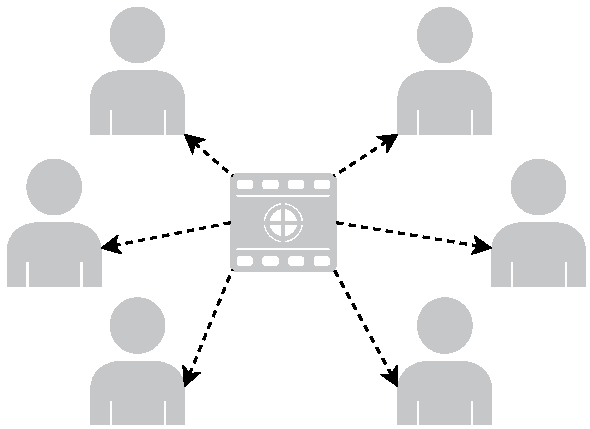
\includegraphics[width=0.5\textwidth]{./figures/star.pdf}
      \caption[One-to-many topology for real time media]{One-to-many topology for real time media.}
	\label{fig:starExample}
\end{figure}

Star scenarios are known as a type of multicast, one source sends the media to the different clients that connect to the origin. When having this topology the common uses rely on video and audio streaming to multiple peers, TV media and streaming conferences are popular use cases.

Some of the problems are: high dependency of the central node and in case of failure of the central node video streaming will stop and all the connectivity with the peers will be over. On the other side, this topology is also good as it provides reliability in case of failure of one of the connected nodes as the rest of the network won't notice any difference on the streaming. 

For example, we could have a major sport even being retransmitted to the viewers by using one-to-many. Other solutions could cover the use of WebRTC to have a CEO talking to the employees with an HMTL5 web application. Music bands also could take advantage of this scenario by being able to transmit his show to the audience with feedback from them in real time. All the previous examples will take advantage of WebRTC by having direct communication from the connected nodes, actual media streaming technologies do not provide this kind of communication between the viewer and the origin.

%\subsubsection{Challenges}
In this topology we will have a video, audio and data streaming connection from one source to multiple devices. This will cause a huge load on the source when having multiple {\it PeerConnection} running, central node performance will be a big constraint in this topology. 

Observing other topologies, in this case, media delay on the network is not as important as other options due to the one-way communication only, in some scenarios video and audio is not required to be received on the source so having the media delayed a couple of seconds is not going to affect the user experience in the call.

From the client perspective, the {\it PeerConnection} stablished will be easy to handle as  in most cases no streams will be sent back to the source, except the RTCP messages and possible data.

\subsection{Many-to-Many}

Many-to-many topologies are also known as mesh, this style of topology is used in multiple VoIP systems for conferencing purposes. Conferences are used in enterprises for long-distance communication between employees and working groups, by this, the need of having those calls working with good response for all participants is very important.

In a full mesh topology all peers connect between them increasing the number of connections and used resources.

The value of fully meshed networks rely on the number of subscribers, the amount of {\it PeerConnections} stablished in a mesh network will depend on the amount of people in the conference. The number of {\it PeerConnections} will grow rapidly based on Equation~\ref{eq:meshformula}.

\begin{equation}
	\label{eq:meshformula}
	c = \frac{n(n-1)}{2}\\
	
	c \text{: Number of {\it PeerConnections}}\
		
	n \text{: Nodes in the mesh}
\end{equation}

Equation~\ref{eq:meshformula} calculates the amount of WebRTC connections required for a {\it full mesh} topology. 

%Inside the mesh structure we can find other types of topologies such as {\it Multipoint Control Unit (MCU) \nomenclature{MCU}{Multipoint Control Unit}}, {\it hub and spoke}, {\it three} and {\it overlay}.

\subsection{Multipoint Control Unit (MCU) \nomenclature{MCU}{Multipoint Control Unit}}

MCUs is a device used to bridge streams in conferences, it multiplexes, mixes and encodes media of different sources to be sent over one gateway. MCU usage will be a good alternative when designing WebRTC infrastructures, the ability to multiplex different streams into the same channel will directly affect on how the client performs when reproducing the video reducing the amount of used resources. 

In real time media topologies MCU is a common component, used as relay it helps end devices to handle less load for the sources by multiplexing all the streams of the call into the same channel, we can have multiple peers connected to the same MCU that will multiplex the media sent by them into one stream forwarded to all the participants.

Some MCUs may have to encode and decode media on the fly, this is can be difficult in real time applications but can provide different encoding options to adapt the output to the link conditions.

Drawbacks on the MCU model rely on the dependency of the end nodes from the MCU, if the MCU fails to give good latency and performance the call quality will be affected and receivers won't get the expected response. Load in the MCU can be very high when multiple conferences are being stablished, this will require abundant resources and good throughput.

\subsection{Overlay}

Overlaying media streams is the ability of a peer to forward media to a third party. Topologies that use overlay are those that require the media to be forwarded from one peer to the other, this kind of behavior is given in multiple peer topologies such as {\it hub and spoke} or {\it tree} seen in Figure~\ref{fig:overlaytopologies}.

Generally, in multiple peer scenarios we can combine all of the following structures to build a topology that fit our requirements.

WebRTC does not provide native support for media overlay but it is planned to implement those features in future versions of the API. Traditionally overlay has been used for media streaming over the internet.

\begin{figure}[h]
        \centering
        \begin{subfigure}[b]{0.5\textwidth}
                \centering
                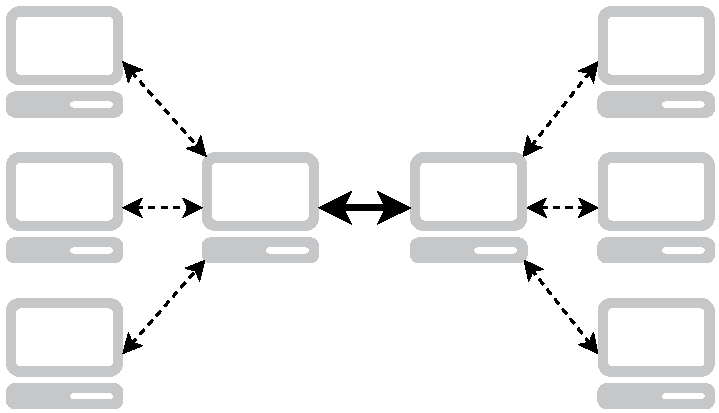
\includegraphics[width=\textwidth]{./figures/hubandspoke.pdf}
                \caption{Spoke-hub topology}
                \label{fig:hubandspoke}
        \end{subfigure}%
        ~ %add desired spacing between images, e. g. ~, \quad, \qquad etc.
          %(or a blank line to force the subfigure onto a new line)
        \begin{subfigure}[b]{0.5\textwidth}
                \centering
                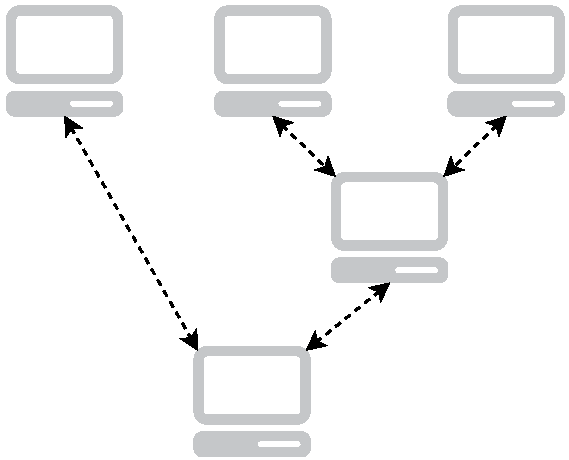
\includegraphics[width=\textwidth]{./figures/three.pdf}
                \caption{Tree topology}
                \label{fig:three}
        \end{subfigure}
        \caption[Overlay topologies]{Overlay topologies.}
        \label{fig:overlaytopologies}
\end{figure}

\subsubsection{Spoke-hub}

Spoke-hub distribution is a topology composed by nodes and arranged like a chariot wheel. Traffic moves along spokes that are connected to the hub at the center. This type of topology, represented in Figure~\ref{fig:hubandspoke}, is good as it requires less connections to perform a full mesh communication in the network. 

This is a centralized model, we might have problems if the key nodes of the topology are fail. It also relies in one or multiple trunk paths that can be crucial for the success of the streaming, those paths should provide good throughput and low delay.

In some technologies that rely in hub and spoke the central nodes are usually picked from the end users, calculating the best response from the users the topology is able to select the optimal candidate where the rest of nodes will connect to. When this happens that node is handling and forwarding more data that in a standalone call.

This topology uses the concept of overlay previously described.

Spoke-hub concept is also used for logistics in the world for delivering products and goods around the globe, focusing in bridges over the continents goods in Europe are distributed within an internal network and shipped to other continents from a centralized node.  

\subsubsection{Tree}
 
Tree topology is based on a node hierarchy, the highest level of the tree consist of a single node that is connected to one or more nodes that forward the traffic to the other layers of the topology. Tree topologies are not constrained by the amount of levels and can adapt to the required amount of end users as seen in Figure~\ref{fig:three}.  

This type of topologies are scalable and manageable. In case of failure it is relatively easy to identify the broken branch of the tree and repair that node.

On the other side, we will have connectivity problems if a node fails to keep the link up, all the layers under that node will be affected and the media forwarding will stop.

Overlay is crucial for this topology that is widely used in media streaming, for real time communications large tree topologies won't be the best candidates given the delay produced when forwarding the packets.

Topologies such as tree are not only used for media streaming but they can also be used to provide wireless coverage in difficult areas, acting as hotspots, each hop can extend the coverage of the wireless in remote areas.


%\subsubsection{Challenges}
%
%When running multiple peer connections browsers on the client side will be obliged to handle multiple incoming streams and keep up all the connections stablished, this will be a problem regarding to the resources on the client side. 
%
%So, alongside with other problems mentioned in previous topologies, resources will directly affect on how this scenario performs in different users. 
%
%On the other side, even considering that NAT and Firewall connectivity issues are solved, we should be careful when guaranteeing all peer connections to be correctly stablished. TURN/STUN failures might directly affect to the success ratio in this topology.

